\section{202109-4 收集卡牌}
	\begin{itemize}
		\item 时间限制:$1.0\texttt{ s}$.
		\item 空间限制:$512.0\texttt{ MiB}$.
	\end{itemize}
	\subsection{题目}
		\subsubsection{题目描述}
			\par 小林在玩一个抽卡游戏,其中有 $n$ 种不同的卡牌,编号为 $1$ 到 $n$。每一次抽卡,她获得第 $i$ 种卡牌的概率为 $p_i$。如果这张卡牌之前已经获得过了,就会转化为一枚硬币。可以用 $k$ 枚硬币交换一张没有获得过的卡。
			\par 小林会一直抽卡,直至集齐了所有种类的卡牌为止,求她的期望抽卡次数。如果你给出的答案与标准答案的绝对误差不超过 $10^{-4}$,则视为正确。
			\par 提示:聪明的小林会把硬币攒在手里,等到通过兑换就可以获得剩余所有卡牌时,一次性兑换并停止抽卡。
		\subsubsection{子任务}
			\par 对于 $20\%$ 的数据,保证 $1\leq n,k\leq 5$。
			\par 对于另外 $20\%$ 的数据,保证所有 $p_i$ 是相等的。
			\par 对于 $100\%$ 的数据,保证 $1\leq n\leq 16$,$1\leq k\leq 5$,所有的 $p_i$ 满足 $p_i\geq\frac{1}{1000}$ 且 $\sum\limits_{i=1}^np_i=1$。
	\subsection{解法 A(20 分)}
		\subsubsection{原理阐释}
			\par 我们考虑设计状态 $f_{a_1,\cdots,a_n}$ 表示抽到第 $i$ 种卡牌 $a_i$ 次对应的概率,则状态转移方程为
			$$f_{a_1,\cdots,a_i,\cdots,a_n}=\sum\limits_{i=1}^n[a_i\geq 1]f_{a_1,\cdots,a_i-1,\cdots,a_n}p_i$$
			边界条件为
			$$f_{0,\cdots,0}=1$$。
			\par 对于状态 $f_{a_1,\cdots,a_n}$,总的抽卡次数 $\text{tot}=\sum\limits_{i=1}^na_i$,抽到有用卡牌(没有变成硬币)数目为 $\text{cnt}=\sum\limits_{i=1}^n[a_i\neq 0]$,从而硬币数目 $\text{coin}=\text{tot}-\text{cnt}$。
			\par 此时答案的计算式可导出为
			$$\mathbb{E}=\sum\limits_{\text{coin}\geq (n-\text{cnt})\times k}f_{a_1,\cdots,a_n}\text{tot},$$
			代入以上表达式,即得计算式
			$$\mathbb{E}=\sum\limits_{\left(\sum\limits_{i=1}^na_i-\sum\limits_{i=1}^n[a_i\neq 0]\right)\geq \left(n-\sum\limits_{i=1}^n[a_i\neq 0]\right)\times k}\left(f_{a_1,\cdots,a_n}\sum\limits_{i=1}^na_i\right).$$
			\par 递推过程的时间复杂度为 $\Theta((nk)^n)$,求答案过程的时间复杂度为 $((nk)^n)$,空间复杂度为 $\Theta((nk)^n)$。
	\subsection{解法 B(40 分)}
		\subsubsection{原理阐释}
			注意到 $p_i$ 全相等($=\frac{1}{n}$),从而对于解法 A 中的 $f_{a_1,\cdots,a_n}$,我们由多重排列公式可以有
			$$f_{a_1,\cdots,a_n}=\frac{\left(\sum\limits_{i=1}^na_i\right)!}{\prod\limits_{i=1}^n(a_i!)}p^{\sum\limits_{i=1}^na_i}.$$
			代入求答案表达式可以得出解法,不具有一般性,故此处不再赘述。
		\subsubsection{C++ 代码实现}
	\subsection{解法 C(100 分)}
		\subsubsection{原理阐释}
			\par 之所以我们的算法不够优秀,是因为状态设计的问题,我们从状态设计重新入手,设计一个优秀的状态。
			\par 注意到抽到过一次某种卡牌后,我们再抽到它不论多少次都会变成硬币,因此我们发现,对于一张卡牌,重要的是有没有抽到过,对于整个过程,重要的是有多少个硬币。
			\par 从而设计状态 $f_{i,\mathbf{S}}$,表示抽卡 $i$ 次,抽到卡牌的集合二进制表示为 $\mathbf{S}$ 的概率,则已经抽到卡牌的数量即为 $\operatorname{cnt}(\mathbf{S})$,即 $\mathbf{S}$ 的二进制表示中 $1$ 的个数,抽到硬币的数目即为 $i-\operatorname{cnt}(\mathbf{S})$。
			\par 状态转移方程(贡献形式)为
			$$f_{i,\mathbf{S}}\to_{j=1}^n f_{i+1,\mathbf{S}\cup\{j\}}p_j,$$
			边界条件为
			$$f_{0,\varnothing}=1.$$
			答案计算式同解法 A,化为
			$$\mathbb{E}=\sum\limits_{i-\operatorname{cnt}(\mathbf{S})\geq\left(n-\operatorname{cnt}(\mathbf{S})\right)\times k}f_{i,\mathbf{S}}i.$$
			\par 算法的时间复杂度为 $\Theta(n^2k2^n)$,空间复杂度为 $\Theta(nk2^n)$。
			\par 值得注意的是,本题不提供 ``Special Judge'',且要求输出到小数点后 $10$ 位,此时浮点精度难以保证。因此,为了保障浮点精度,我们需要认清浮点数加法不满足加法交换律这一特性,选择最佳的答案求和顺序。
			\par 最简单的是将答案的每一项从小到大排序后再相加,此时精度比较高,可以满足题目的精度需要,额外添加了排序的复杂度(使得代码运行时间从 $60\texttt{ ms}$ 增加到 $120\text{ ms}$ 左右)。
			\par 最准确的是将答案的每项存储在堆中,每次提取最小的两个相加后放回,虽复杂度与排序法一致但常数颇高(实际运行时间 $300\texttt{ ms}$ 左右),故不采用。
			\par 此外还有两种令人诟病的方式,一是换用 ``long double'',但这平添了不必要的时空负担,二是网上代码常见的交换循环顺序,这实际上是不通用且不负责任的做法。
		\subsubsection{C++ 代码实现}
			\par 为提高浮点精度,使用排序升序相加的方法。
			\lstinputlisting[
				style=C++,
				title={\bf 202109-4.cpp},
				tabsize=4
			]{202109-4.cpp}
		\subsubsection{提交结果}
			\begin{figure*}[htbp]
				\centering
				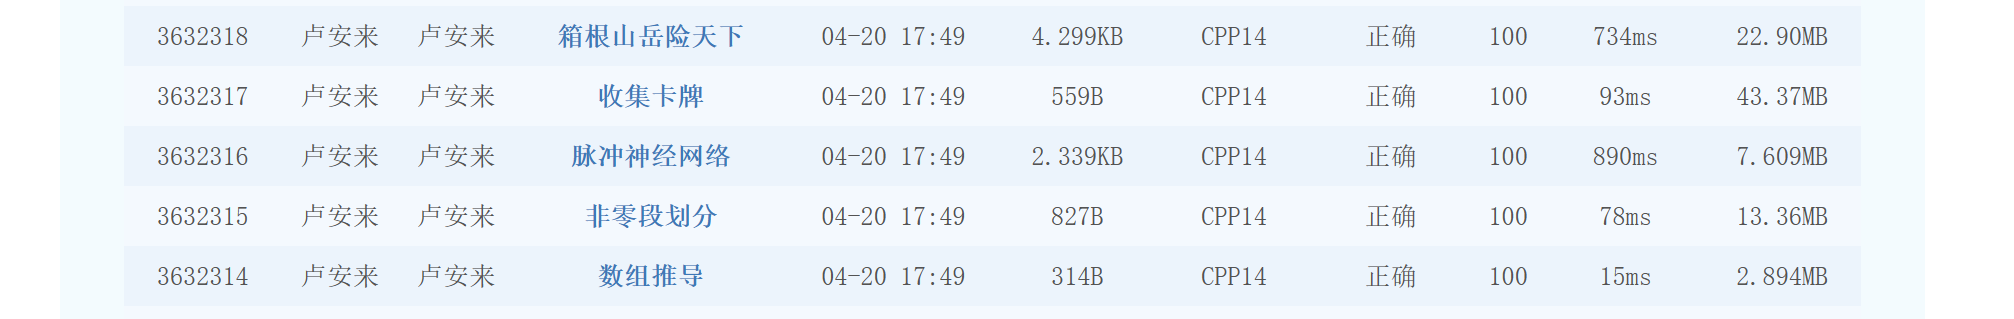
\includegraphics[width=1\textwidth]{result.png}
				\caption{提交结果}
			\end{figure*}
